\documentclass[12pt]{article}
\usepackage[left=3cm, right=3cm, top=3cm]{geometry}
\usepackage{amsmath}
\usepackage{graphicx}
\usepackage{hyperref}
\usepackage{subcaption}
\usepackage{wrapfig}
\usepackage[latin1]{inputenc}

\setlength{\parindent}{0cm}

\title{ECEN303 Lab 5 - Filters}
\author{Celine Jane  300400152}

\begin{document}
	\maketitle
	\section{VCSC Filters}
	\begin{wrapfigure}{l}{0.5\textwidth}
		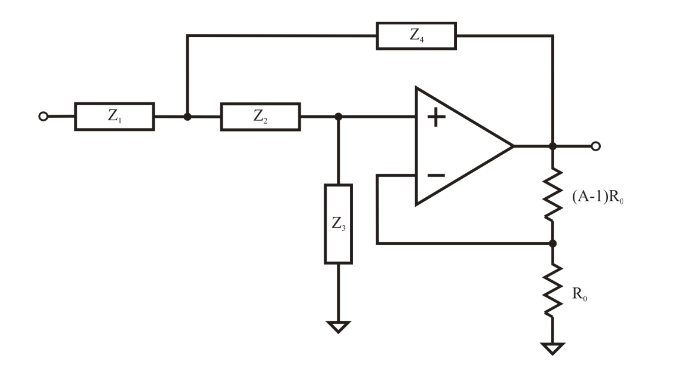
\includegraphics[width=0.5\columnwidth]{Capture}
		\caption{VCSC Filter}
	\end{wrapfigure}
	For this section, the gain and phase response of Bessel and Chebyshev filters will be analysed. These filters will take the form of the low pass filter circuit in Figure 1. The quality factor, Q, has a distinct value for each filter. Q can be described by the equation
	$$ Q = \frac{1}{3-A}$$\\
		\subsection{Bessel Filter}
		For a Bessel filter, $Q=\frac{1}{\sqrt{3}}$. Using this, A and subsequently $R_{0}$ can be found.
		$$\frac{1}{3-A} = \frac{1}{\sqrt{3}}$$
		$$3-A = \sqrt{3}$$
		$$A = 3 - \sqrt{3} = 1.265$$\\
		$$ (1-A)R_{0} = 0.265R_{0}$$
		$$Picking\quad R_{0} = 3.9K\Omega$$
		$$0.265R_{0} = 1043.25\Omega \simeq 1k\Omega+47\Omega$$ 
		\newpage
		The Bessel filter is designed as follows:
		\begin{figure}[h!]
			\centering
			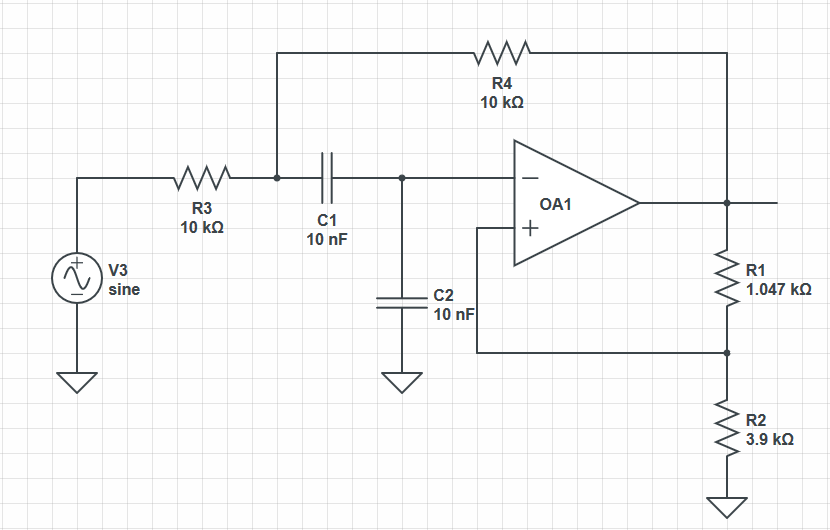
\includegraphics[width=\columnwidth]{bessel}
			\caption{Bessel Filter}
		\end{figure}
	
		The gain and phase responses were found by looking at the output of the circuit as the input signal from a function generator had its frequency increased.\\
		
		\begin{figure}[h!]
			\centering
			\begin{subfigure}[b]{0.45\textwidth}
				\centering
				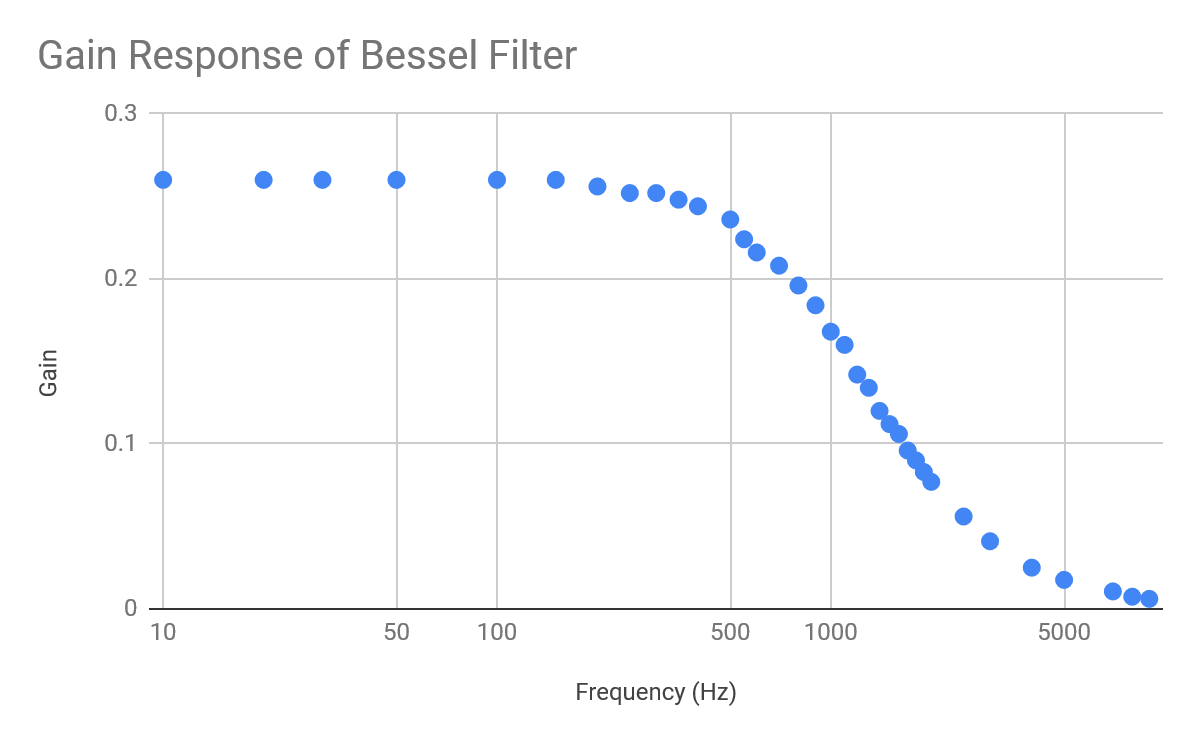
\includegraphics[width=\textwidth]{bessel_gain}
			\end{subfigure}
			\hfill
			\begin{subfigure}[b]{0.45\textwidth}
				\centering
				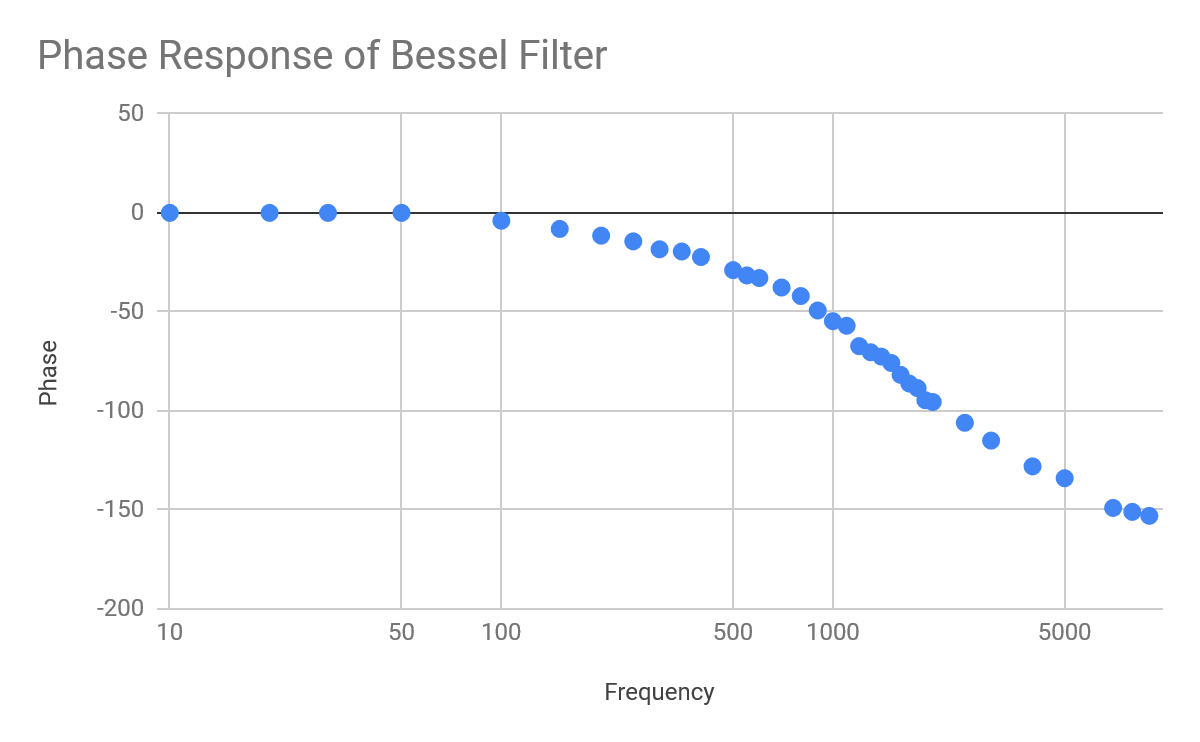
\includegraphics[width=\textwidth]{bessel_phase}
			\end{subfigure}
			\caption{Gain and Phase Response of Bessel Filter}
		\end{figure}
		
		In Figure 3 it can be seen that the cutoff frequency is around 1kHz. At this point the phase also decreases and tends towards $-180$ degrees (instability).
		
		\subsection{Chebyshev Filter}
		A Chebyshev filter has $Q = 0.9564$. The resistances can be found from this:
		$$ 3-A = \frac{1}{0.9564}$$
		$$ A = 3 - 1.04559$$
		$$ A = 1.954 $$\\
		$$ (1-A)R_{0} = 0.954R_{0}$$
		$$Picking\quad R_{0} = 3.9K\Omega$$
		$$0.954R_{0} = 3722.2\Omega \simeq 2.7k\Omega+1k\Omega$$ 	
		The Chebyshev filter is as designed as followed:
		\begin{figure}[h!]
			\centering
			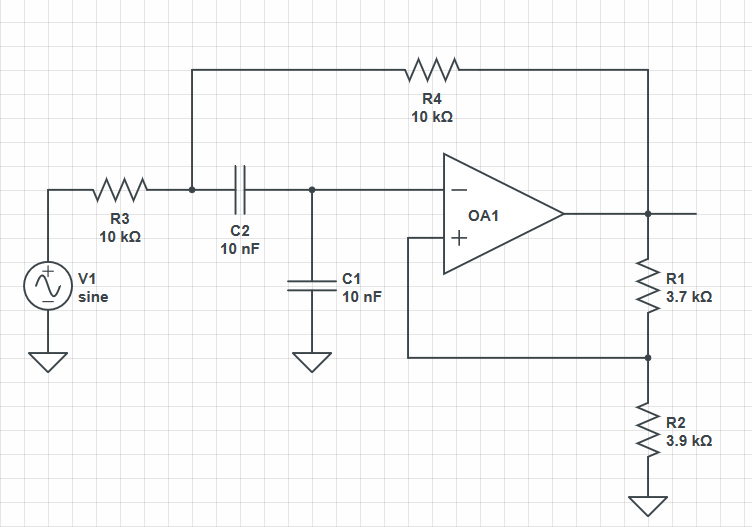
\includegraphics[width=\columnwidth]{Capture2}
			\caption{Chebyshev Filter}
		\end{figure}
		\newpage
		The responses found (in comparison with the Bessel filter) can be seen in Figure 5.\\
				\begin{figure}[h!]
			\centering
			\begin{subfigure}[b]{0.45\textwidth}
				\centering
				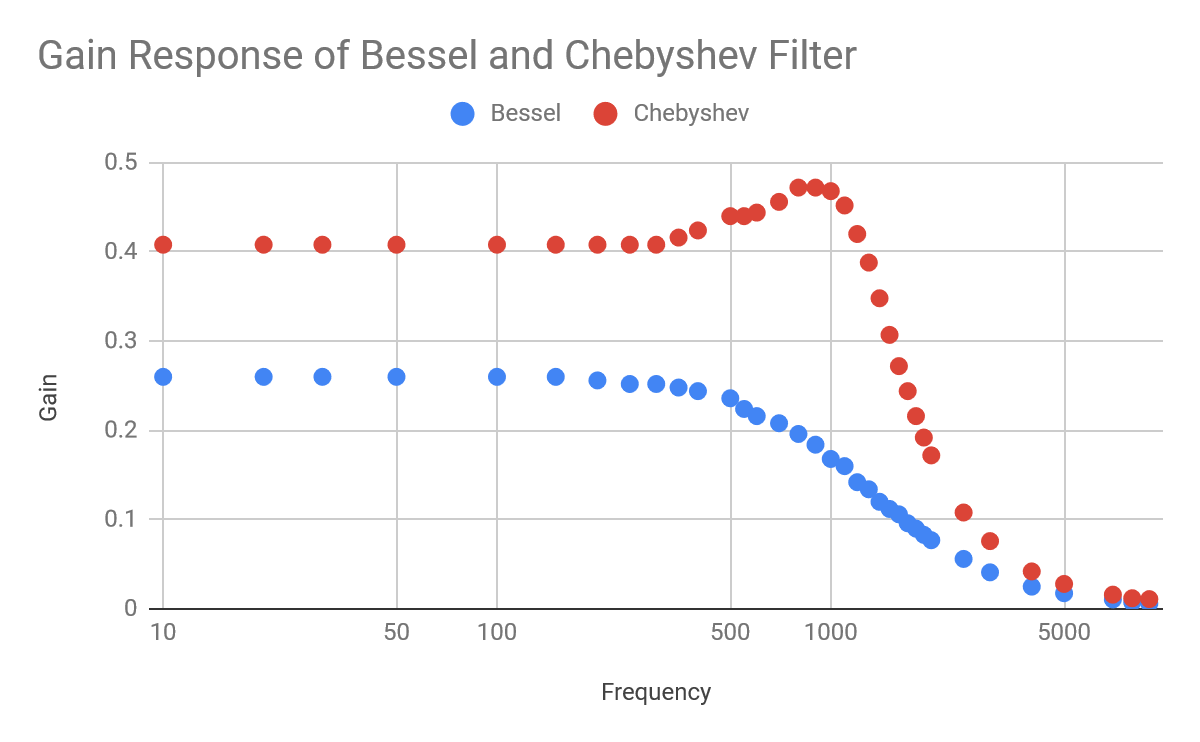
\includegraphics[width=\textwidth]{chebyshev_gain}
			\end{subfigure}
			\hfill
			\begin{subfigure}[b]{0.45\textwidth}
				\centering
				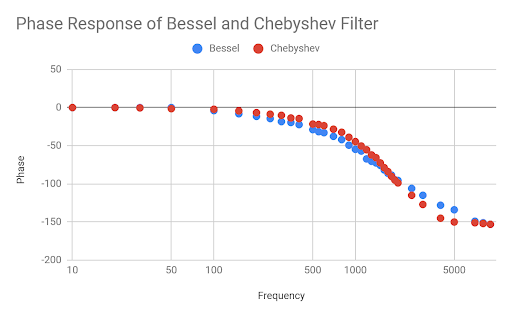
\includegraphics[width=\textwidth]{chebyshev_phase}
			\end{subfigure}
			\caption{Gain and Phase Response of Chebyshev and Bessel Filter}
		\end{figure}
		
		It can be seen that the Chebyshev filter has the same cut off frequency as the Bessel filter at around 1kHz. The gain of the Chebyshev filter is higher than that of the Bessel. However it can be seen that the Chebyshev filter has a ripple just before the cut-off frequency. The Bessel filter is more reliable in frequencies nearer the cutoff frequency. \\
		
		The Chebyshev filter has a smaller phase response for frequencies before the cutoff frequency and a larger phase response after the cutoff frequency.
		
		\subsection{Frequency Scaling Factor (FFS)}
		The FFS can be described via the equation
		$$\omega_{0} = \frac{1}{FSF}\frac{1}{RC}$$
		Both the filters have the same cut-off frequency $2\pi\cdot1000$, so will have the same FSF.
		$$2\pi\cdot1000 = \frac{10000}{FSF}$$
		$$FSF = 1.59$$
		
		\section{Filter Design and Simulation Tools}
		The Butterworth filter has $Q = \frac{1}{\sqrt{2}}$.
		$$ 3-A = \sqrt{2}$$
		$$ A = 3 - \sqrt{2}$$
		$$ A = 1.586 $$\\
		$$ (1-A)R_{0} = 0.586R_{0}$$
		$$Picking\quad R_{0} = 3.9K\Omega$$
		$$0.954R_{0} = 2284.6\Omega \simeq 2.2k\Omega+82\Omega$$\\
		
		The Butterworth filter is designed as follows:\\
		\begin{figure}[h!]
			\centering
			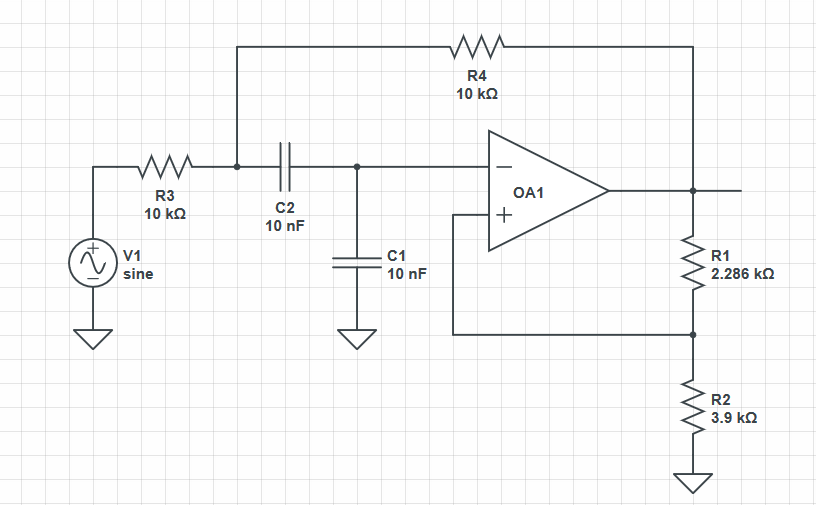
\includegraphics[width=\columnwidth]{butterworth}
			\caption{Chebyshev Filter}
		\end{figure}
		\newpage
		\begin{figure}[h!]
			\centering
			\begin{subfigure}[b]{0.49\textwidth}
				\centering
				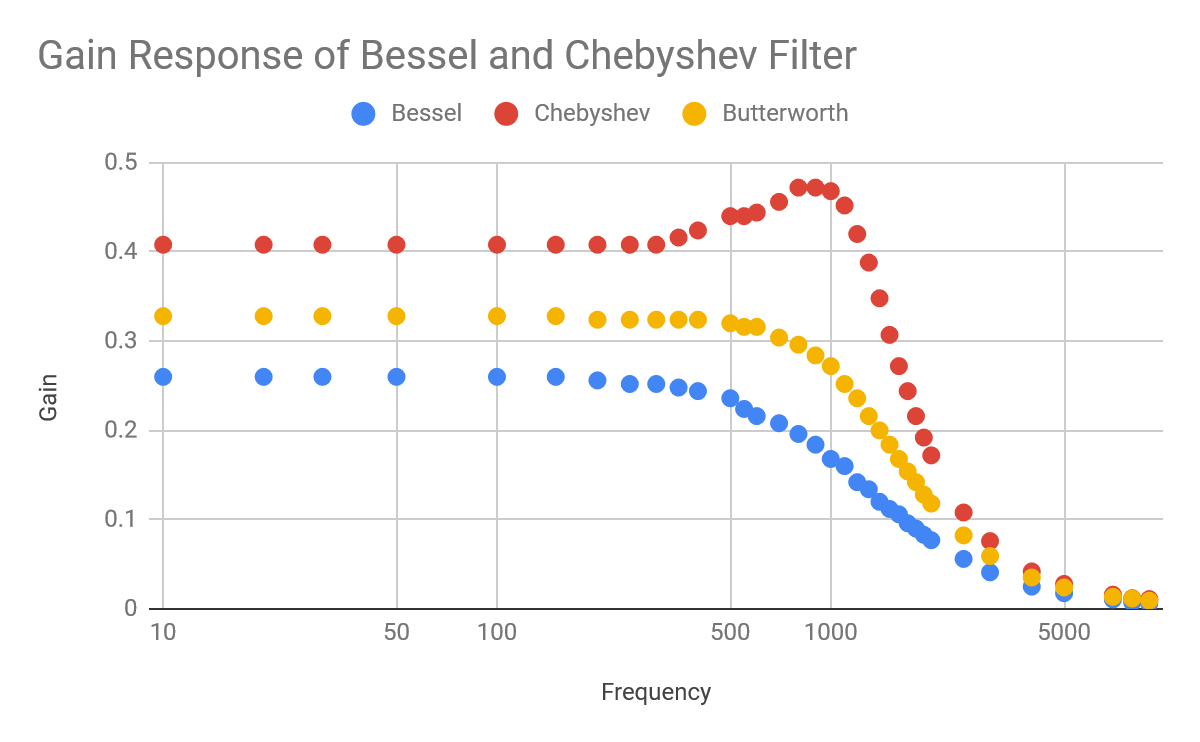
\includegraphics[width=\textwidth]{butterworth_gain}
			\end{subfigure}
			\hfill
			\begin{subfigure}[b]{0.49\textwidth}
				\centering
				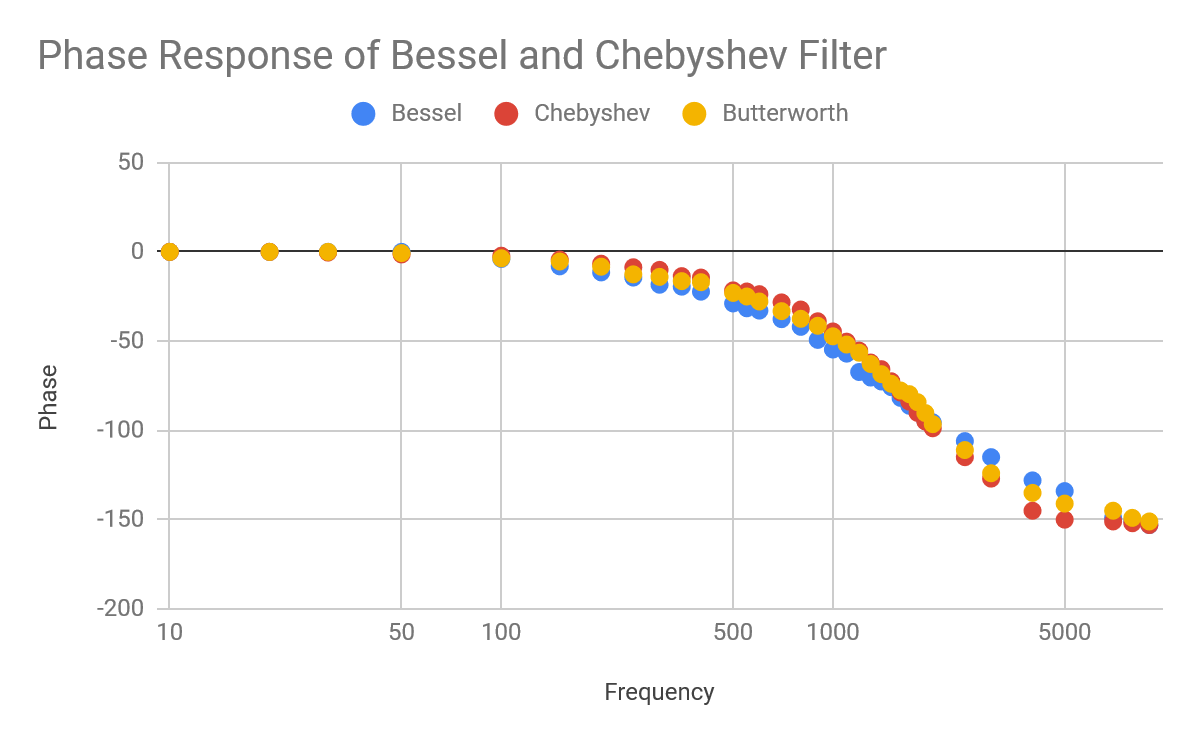
\includegraphics[width=\textwidth]{butterworth_phase}
			\end{subfigure}
			\caption{Gain and Phase Response of Butterworth, Chebyshev and Bessel Filter}
		\end{figure}
	\section{Discussion}
		\subsection{Merits of Different Filters}
		\subsection{Sampling Rate and Bandwidth}
	
\end{document}